\documentclass{standalone}
\usepackage{pgfplots}
\pgfplotsset{compat=1.18} % Adjust this version if needed based on your LaTeX distribution

\begin{document}
	
	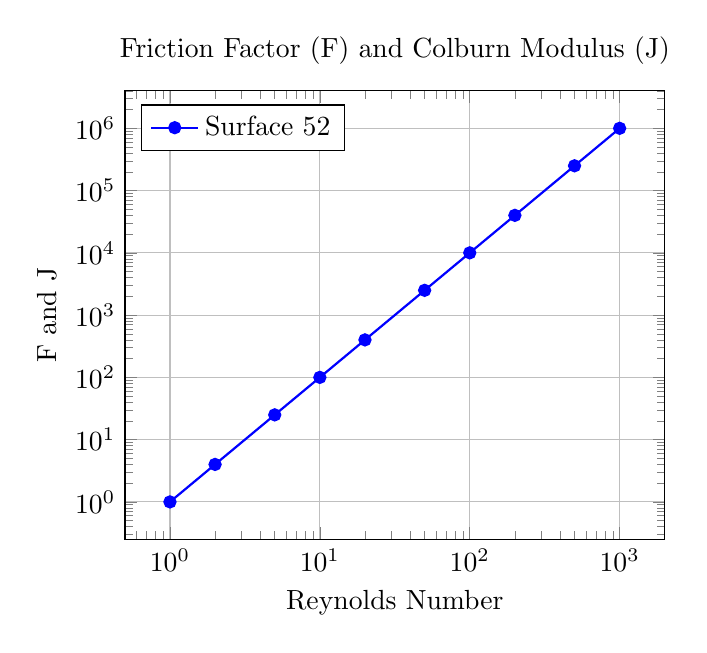
\begin{tikzpicture}
		\begin{loglogaxis}[
			xlabel={Reynolds Number},
			ylabel={F and J},
			grid=major, % Adds a grid for better readability
			title={Friction Factor (F) and Colburn Modulus (J)},
			legend entries={Surface 52},
			legend pos=north west
			]
			% Sample data: 10 (x,y) pairs
			\addplot[
			color=blue,
			mark=*, % Adds markers at data points
			thick
			] coordinates {
				(1, 1)    % Point 1
				(2, 4)    % Point 2
				(5, 25)   % Point 3
				(10, 100) % Point 4
				(20, 400) % Point 5
				(50, 2500)% Point 6
				(100, 10000) % Point 7
				(200, 40000) % Point 8
				(500, 250000) % Point 9
				(1000, 1000000) % Point 10
			};
		\end{loglogaxis}
	\end{tikzpicture}
	
\end{document}